\subsection{The Cleaning Web Service}
\label{sec:cleaningService}

D3.2~\cite{d3.2} described the RESTful API of the cleaning web service. 
The cleaning web service contains the two methods \texttt{getCleaningSuggestions} and \texttt{clean}, to which this deliverable provides an update.
The functionality of the methods, as specified in D3.1~\cite{d3.1}, remains unchanged.

The HTTP method for the \texttt{getCleaningSuggestions} method has been changed from POST to GET, as the method retrieves information from the server, whereas POST is for updating existing resources.  The semantics of the \texttt{getCleaningSuggestions} method does not foresee any manipulation of resources; in our case it merely returns RDF data.
The parameters of the \texttt{getCleaningSuggestions} methods have slightly changed.  The response of the method has been extended to address flows in case of passing illegal or incorrect parameters. The detailed description of the \texttt{getCleaningSuggestions} request and response is provided below.

The implementation of the cleaning part of the exposed web service led to updates of the POST request and response parameters with regard to D3.1~\cite{d3.1}.

The typical usage of the cleaning service follows the workflow outlined for the cleaning application in figure~\ref{fig:workflow}.
The updated user interface is shown in figure~\ref{fig:ui}.

\begin{figure}[ht!]
\centering
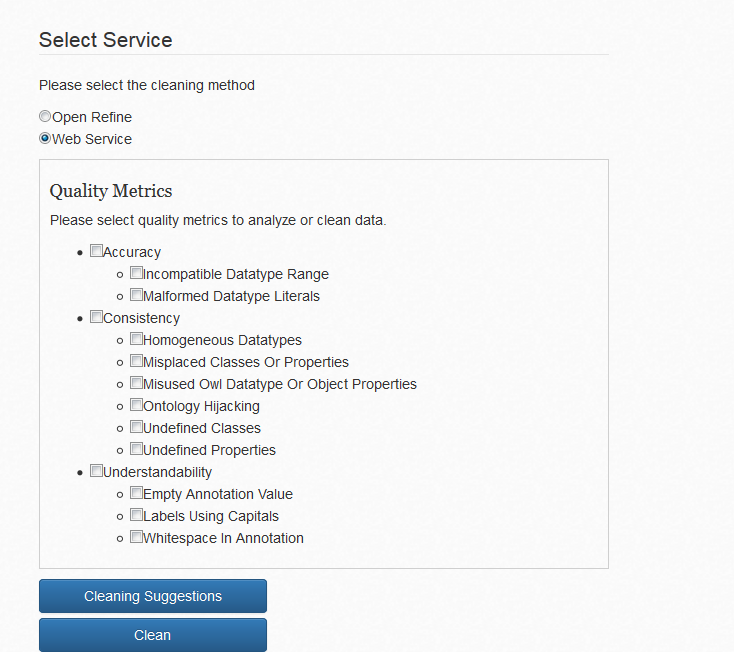
\includegraphics[width=\textwidth]{figures/WebService.png}
\caption{Cleaning process workflow}
\label{fig:ui}
\end{figure}





\subsubsection{Exposed Web Service Interfaces}
\label{sec:service-API}

Table~\ref{tbl:valid_meth} provides an overview of the cleaning methods.

\begin{table}[h]
\captionsetup{justification=raggedright,singlelinecheck=false}
\caption{Cleaning Methods}
\label{tbl:valid_meth}
\begin{tabular}{|p{5cm}|p{10cm}|}
\hline
\multicolumn{2}{|l|}{\textbf{Methods}} \\ \hline

\textbf{Modifier and Type} & 
\textbf{Method and Description} \\ \hline

\texttt{HttpServletRequest} & 
\texttt{getCleaningSuggestionsREST(HttpServletRequest
request, HttpServletResponse response)}: \textbf{GET} method returning a set of cleaning suggestions. \\ \hline

\texttt{HttpServletRequest} & 
\texttt{cleanREST(HttpServletRequest
request, HttpServletResponse response)}: \textbf{POST} method removing triples affected by selected quality problems. \\ \hline

\hline
\end{tabular}
\end{table}
Note: \textit{HttpServletRequest} and \textit{HttpServletResponse} are interfaces in the \textit{javax.servlet.http} package.

\subparagraph{Method Details}

\begin{description}

\item{\textbf{getCleaningSuggestionsREST}:} \textbf{GET} method returning a set of cleaning suggestions.

\textbf{URL (partial):} \url{/quality_extension/get_cleaning_suggestions} 

\textbf{Parameters}: 
\begin{itemize}
\item \texttt{HTTP Request message}: A JSON-encoded string havng the following structure: \\
\hspace*{0.2 cm}\textit{\{}\\
\hspace*{0.5 cm}\textit{"download": "Dataset",} \\
\hspace*{0.5 cm}\textit{"metrics": ["metric1", "metric2"]}  \\
\hspace*{0.2 cm}\textit{\}} \\
\end{itemize}
Where
\begin{description}
\item[download:] The URL of a file to be validated. 
\item[metrics:] A list of quality metrics with respect to which cleaning suggestions should be generated. 
\end{description}


\textbf{Returns}: A Response instance which has a \texttt{JSON}-encoded entity content depending on the input parameter of the method. We distinguish the following cases: 
\begin{itemize}
\item  HTTP status code \texttt{400 Bad Request} and the entity content, if the input parameters or one of them are empty:\\ \hspace*{0.2 cm}\textit{\{}\\
\hspace*{0.5 cm} \textit{"status" : "error",}\\
\hspace*{0.5 cm} \textit{"message" : "Request parameters are not complete."}\\ \hspace*{0.2 cm} \textit{\}}

\item  HTTP status code \texttt{200 OK} and the entity content, if the input parameters are correct and the get cleaning suggestion method has not failed:\\ \hspace*{0.2 cm} \textit{\{}\\
 \hspace*{0.5 cm}\textit{"status" : "ok",}\\ 
 \hspace*{0.5 cm}\textit{"message" : "Quality report in one of the RDF serialisations."}\todo{CL: how do you specify the desired serialisation in the request?} \\ \hspace*{0.2 cm} \}

\item HTTP status code \texttt{400 Bad Request} and the entity content, if the input parameters are not correct:\\ \hspace*{0.2 cm} \textit{\{} \\
\hspace*{0.5 cm} \textit{"status" : "error",}\\
\hspace*{0.5 cm}  \textit{"message" : "Request parameters cannot be parsed."}\\ \hspace*{0.2 cm} \textit{\}}

\end{itemize}
The cleaning report is created according to the QR (Quality Report) and QPROB (Quality Problems) ontologies presented in D3.2~\cite{d3.2}.
An example of the cleaning report is shown in Figure~\ref{lst:cleaning_report}.


We also extended the cleaning report by statistics that summarize information about identified quality problems and affected triples. 
The QR ontology has been extended by the corresponding classes and properties represented in Figure~\ref{fig:stat}.


\begin{figure}[ht!]
\centering
% left bottom right top
\includegraphics[page=8,trim=1.0cm 16.0cm .8cm 1.0cm,clip,width=\textwidth]{figures/CleaningFigures.pdf}
\caption{Quality Statistics in Quality Report Ontology}
\label{fig:stat}
\end{figure}
\lstinputlisting[caption={An example of a cleaning report},label=lst:cleaning_report]{figures/cleaning_report.trig}\todo{CL: I don't understand the first triple.}\todo{CL: The objects of the \textit{rdf:predicate} and \textit{rdf:subject} triples were given as strings; however these should really be URIs.  I have fixed this in the listing, but please make sure the implementation also uses URIs here.}.


\item{\textbf{clean}:} a \textbf{POST} method to clean a dataset by applying the rule ``delete every triple that is affected by a quality problem w.r.t.\ at least one of the metrics specified''.

\textbf{URL (partial):} \url{/quality_extension/clean} 

\textbf{Parameters}: 
\begin{itemize}
\item \texttt{HTTP Request message}: A JSON-encoded string of the following structure: \\
\textit{\{} \\
\hspace*{0.5 cm}\textit{"download": "Dataset",} \\
\hspace*{0.5 cm}\textit{"metrics": ["metric1", "metric2"],} \\
\hspace*{0.5 cm}\textit{"delta": "true | false"} \\  
\textit{\}} \\

Where 
\begin{description}
\item[Dataset:] The URI of an \texttt{RDF} file to be validated. 
\item[metrics:] A list of metrics with respect to which cleaning suggestions should be generated.
\end{description}

\end{itemize}
\textbf{Returns}: A Response instance which has a JSON encoded entity content depending on the input parameter of the method. We distinguish the following cases: 
\begin{itemize}
\item  HTTP status code \texttt{400 Bad Request} and the entity content, if the input parameters or one of them are empty:\\ \hspace*{0.2 cm}\textit{\{}\\
\hspace*{0.5 cm} \textit{"status" : "error",}\\
\hspace*{0.5 cm} \textit{"message" : "Request parameters are not complete."}\\ \hspace*{0.2 cm} \textit{\}} 

\item HTTP status code \textit{400 Bad Request} and the entity content, if the input parameters are not correct:\\ \hspace*{0.2 cm} \textit{\{} \\
\hspace*{0.5 cm} \textit{"status" : "error",}\\
\hspace*{0.5 cm}  \textit{"message" : "Request parameters cannot be parsed or an error occurred while applying metrics."}\\ \hspace*{0.2 cm} \textit{\}}

\item  HTTP status code \textit{200 OK} and the entity content, if the input parameters are correct and the getCleaningSuggestion method has not failed: \\ \hspace*{0.2 cm} \textit{\{}\\ \hspace*{0.5 cm} \textit{"status" : "ok",}\\ \hspace*{0.5 cm} \textit{"uri":  "Cleaned \texttt{RDF} data serialized in Turtle.",}\todo{CL: Why just Turtle here, when other methods support more serialisations?} \\ \hspace*{0.5 cm}\textit{"delta" : "Removed \texttt{RDF} statements serialized in Turtle."} \\ \hspace*{0.2 cm}\textit{\}} 
\end{itemize}

A further improvement planned for the near future is not to return serialised RDF data, but to implement a server-side ``assets store'' within the extension, to which additional REST methods would enable access.
Once this is done, it would be sufficient for the \textit{clean} method to merely return the URL of the cleaned dataset, which the client would then download from the assets store.
\end{description}

%%% Local Variables: 
%%% mode: latex
%%% TeX-master: "D3.3"
%%% End: 
